
% This LaTeX was auto-generated from MATLAB code.
% To make changes, update the MATLAB code and republish this document.

\documentclass{article}
\usepackage{graphicx}
\usepackage{color}

\sloppy
\definecolor{lightgray}{gray}{0.5}
\setlength{\parindent}{0pt}

\begin{document}

    
    \begin{verbatim}
k=0;
Error=zeros(16,3);
while k<=15
    h=1.6/(2^k);
    data=Euler(0,1.6,0,h);
    Error(k+1,:)=[h,data(end,4),0];
    data=RK4(0,1.6,0,h);
    Error(k+1,3)=data(end,4);
    k=k+1;
end
digits(5)
disp(Error)
latex(sym(vpa(Error)))
logError=log(abs(Error));
meanError=mean(logError);

scatter(logError(:,1),logError(:,2))
hold on
x=xlim;
plot(linspace(x(1),x(2)),linspace(x(1),x(2))+meanError(2)-...
    meanError(1))
% Adds labels and saves the image
legend({'Data','y=x+a'},'location',...
    'northwest')
title('Euler Error as h decreases')
xlabel('log(h)')
ylabel('log(|E_{n}|)')
print('Image_4_1','-depsc')

figure
scatter(logError(:,1),logError(:,3))
hold on
x=xlim;
plot(linspace(x(1),x(2)),4*linspace(x(1),x(2))+meanError(3)-...
    4*meanError(1))
%Adds labels and saves the image
legend({'Data','y=4x+b'},'location',...
    'northwest')
title('Runge-Kutta Error as h decreases')
xlabel('log(h)')
ylabel('log(|E_{n}|)')
print('Image_4_2','-depsc')




function data = Euler(x_0,x_n,y_0,h)
%Creates a table to be filled
    data=zeros(ceil((x_n-x_0)/h)+1,5);
    data(1,:)=[x_0,y_0,y(x_0),y_0-y(x_0),0];
    counter=2;
%Iterates through the rows filling them
    while counter<=ceil((x_n-x_0)/h)+1
        data(counter,:)=[(counter-1)*h+x_0,...
            data(counter-1,2)+h*f((counter-2)*h+x_0,data(counter-1,2)),...
            y((counter-1)*h+x_0),...
            data(counter-1,2)+h*f((counter-2)*h+x_0,data(counter-1,2))-...
            y((counter-1)*h+x_0),...
            (data(counter-1,2)+h*f((counter-2)*h+x_0,data(counter-1,2))-...
            y((counter-1)*h+x_0))/data(counter-1,4)];
        counter=counter+1;
    end
end

function data = RK4(x_0,x_n,y_0,h)
%Follows a similar idea to the Euler function
    data=zeros(ceil((x_n-x_0)/h)+1,5);
    data(1,:)=[x_0,y_0,y(x_0),y_0-y(x_0),0];
    counter=2;
    while counter<=ceil((x_n-x_0)/h)+1
        k1=h*f((counter-2)*h+x_0,data(counter-1,2));
        k2=h*f((counter-2+1/2)*h+x_0,data(counter-1,2)+1/2*k1);
        k3=h*f((counter-2+1/2)*h+x_0,data(counter-1,2)+1/2*k2);
        k4=h*f((counter-2+1)*h+x_0,data(counter-1,2)+k3);
        data(counter,:)=[(counter-1)*h+x_0,...
            data(counter-1,2)+1/6*(k1+2*k2+2*k3+k4),...
            y((counter-1)*h+x_0),...
            data(counter-1,2)+1/6*(k1+2*k2+2*k3+k4)-y((counter-1)*h+x_0),...
            (data(counter-1,2)+1/6*(k1+2*k2+2*k3+k4)-y((counter-1)*h+x_0))/...
            data(counter-1,4)];
        counter=counter+1;
    end
end

%These two functions were created to stop repeatedly defining them in the
%above
function z = f(x,y)
    z = -4*y+4*exp(-2*x);
end

function z = y(x)
    z= -2*exp(-4*x)+2*exp(-2*x);
end
\end{verbatim}

        \color{lightgray} \begin{verbatim}          1.6       6.3218      -51.339
          0.8      -6.4721      -4.2435
          0.4     -0.21366   0.00095115
          0.2   -0.0088704   0.00010423
          0.1    -0.004174   5.5117e-06
         0.05     -0.00195   3.1351e-07
        0.025  -0.00093479   1.8658e-08
       0.0125  -0.00045677   1.1374e-09
      0.00625  -0.00022566     7.02e-11
     0.003125  -0.00011215   4.3599e-12
    0.0015625    -5.59e-05   2.7156e-13
   0.00078125  -2.7907e-05   1.6889e-14
   0.00039063  -1.3943e-05    1.138e-15
   0.00019531  -6.9686e-06   3.1919e-16
   9.7656e-05  -3.4836e-06  -6.9389e-17
   4.8828e-05  -1.7416e-06   2.7756e-16


ans =

    '\left(\begin{array}{ccc} 1.6 & 6.3218 & -51.339\\ 0.8 & -6.4721 & -4.2435\\ 0.4 & -0.21366 & 0.00095115\\ 0.2 & -0.0088704 & 0.00010423\\ 0.1 & -0.004174 & 5.5117e-6\\ 0.05 & -0.00195 & 3.1351e-7\\ 0.025 & -0.00093479 & 1.8658e-8\\ 0.0125 & -0.00045677 & 1.1374e-9\\ 0.00625 & -0.00022566 & 7.02e-11\\ 0.003125 & -0.00011215 & 4.3599e-12\\ 0.0015625 & -0.0000559 & 2.7156e-13\\ 0.00078125 & -0.000027907 & 1.6889e-14\\ 0.00039062 & -0.000013943 & 1.138e-15\\ 0.00019531 & -6.9686e-6 & 3.1919e-16\\ 0.000097656 & -3.4836e-6 & -6.9389e-17\\ 0.000048828 & -1.7416e-6 & 2.7756e-16 \end{array}\right)'

\end{verbatim} \color{black}
    
\includegraphics [width=4in]{Question_4_1_01.eps}

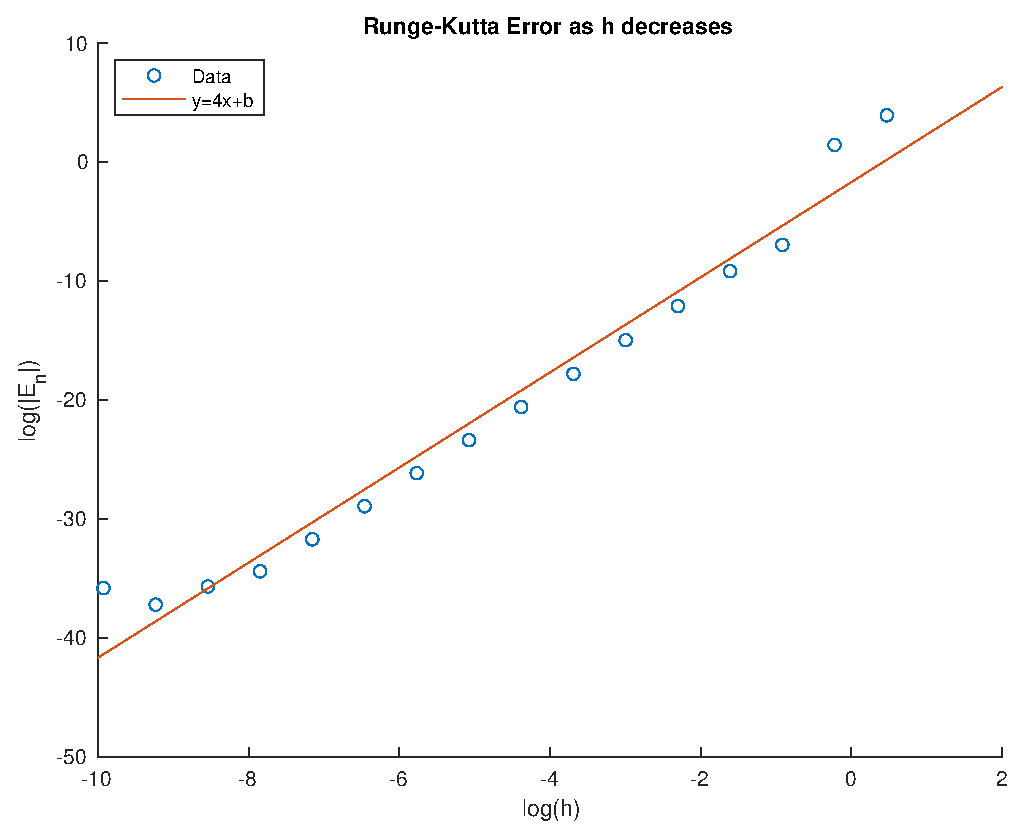
\includegraphics [width=4in]{Question_4_1_02.eps}



\end{document}
    
